\section{Existing Amateur Solutions for Environmental Mapping}
\label{sec:amateur_solutions}
\subsection{Using a Single-Point \gls{lidar} module}

One of the most straightforward approaches to achieve 360° environmental mapping is to utilise a single-point \gls{lidar} module mounted on a platform which can rotate and tilt. 
The implementation could be found in \cite{lidar_design_1}.
\begin{figure}
    \centering
    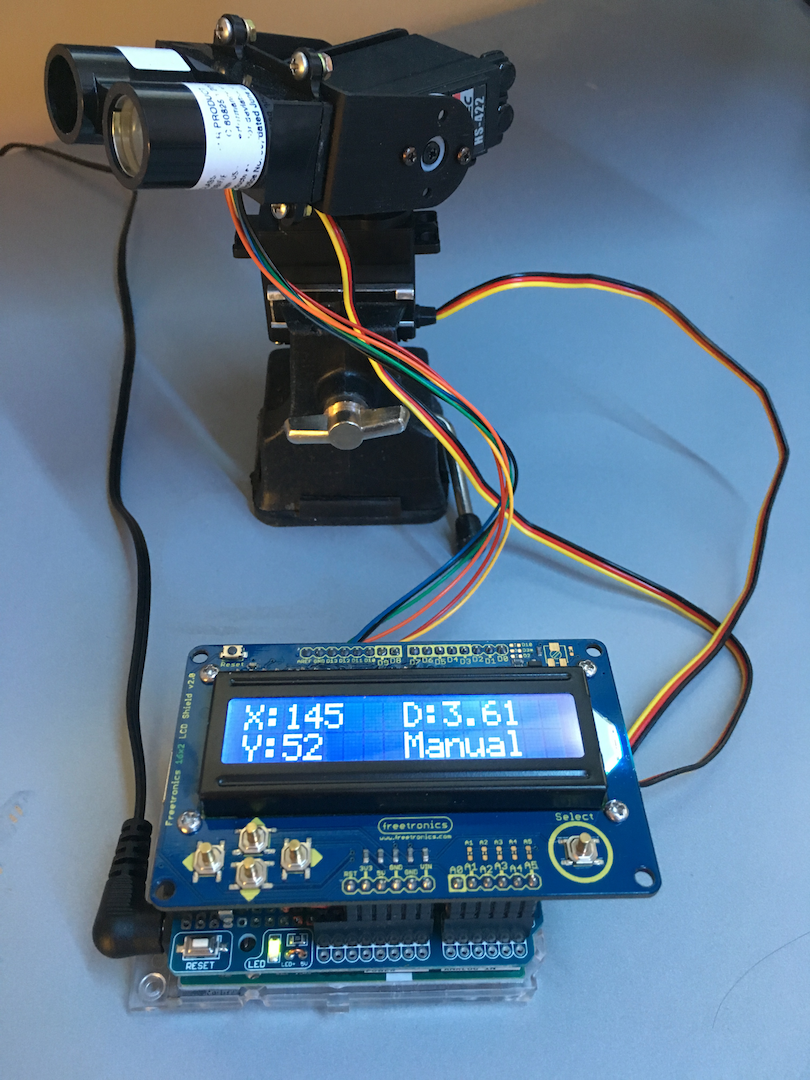
\includegraphics[width=0.5\textwidth]{design/existing_solutions/3D_1.png}
    \caption{Implementation in project \cite{lidar_design_1} using a single-point \gls{lidar}}
    \label{ph:lidar_design_1}
\end{figure}


\begin{tabular}{p{0.45\linewidth} p{0.45\linewidth}}
\textbf{Pros} & \textbf{Cons} \\
\begin{itemize}[label=\textcolor{green!60!black}{\textbf{+}}]
    \item Single-point \gls{lidar}s are the most cost-effective among all existing types
    \item Simple design
\end{itemize}
&
\begin{itemize}[label=\textcolor{red!70!black}{\textbf{--}}]
    \item Slow data acquisition relative to methods leveraging 2D \gls{lidar}'s speed
    \item Movement of lidar may introduce inaccuracies in distance measurements, which need to be compensated for in code if we want to assume that all points are measured from a single position in space
\end{itemize}
\end{tabular}


\subsection{Using a Single-Point \gls{lidar} and a Mirror}
The following approach was used in \cite{lidar_design_2}. A single-point \gls{lidar} is placed below a rotating mirror, which reflects the laser beam horizontally. 
As the mirror rotates, the laser beam scans the environment in 360-degree sweep. 
Moreover, by tilting the mirror at an angle, vertical scanning can also be achieved, allowing for the acquisition of the whole scene.

\begin{figure}
    \centering
    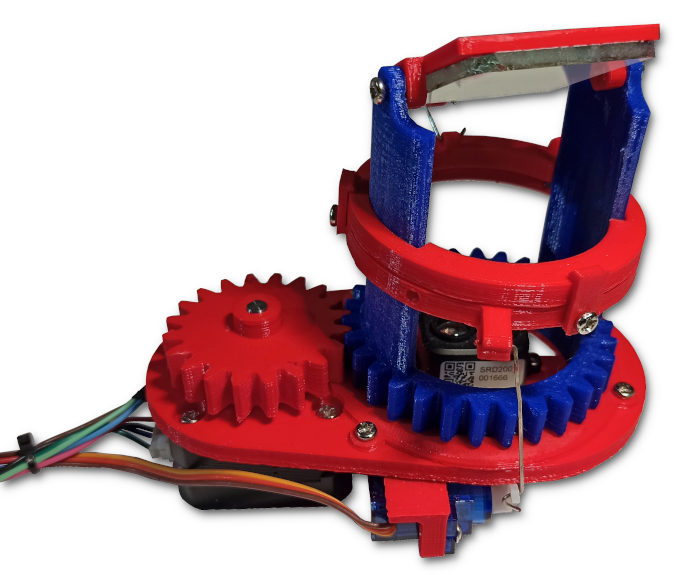
\includegraphics[width=0.75\textwidth]{design/existing_solutions/3D_2.jpg}
    \caption{Implementation in project \cite{lidar_design_2} using a single-point \gls{lidar} and a mirror}
    \label{ph:lidar_design_2}
\end{figure}

\begin{tabular}{p{0.45\linewidth} p{0.45\linewidth}}
\textbf{Pros} & \textbf{Cons} \\
\begin{itemize}[label=\textcolor{green!60!black}{\textbf{+}}]
    \item Cost-effectiveness as in previous implementation
    \item Simple design
    \item Much easier to correct the distance measurement since the \gls{lidar} is stationary and the distance from it to the mirror is known.
\end{itemize}
&
\begin{itemize}[label=\textcolor{red!70!black}{\textbf{--}}]
    \item Slow data acquisition relative to methods leveraging 2D \gls{lidar}'s speed
    \item Mirror quality may affect the accuracy of distance measurements
    \item Mechanical structure holding the mirror may introduce vibrations, thus affecting measurement accuracy
\end{itemize}
\end{tabular}


\subsection{Using a 2D \gls{lidar} Mounted on a Tilting Platform}
\label{sec:tilting_platform}
This approach utilises a 2D \gls{lidar} sensor mounted on a platform that can tilt the sensor side to side, as demonstrated in \cite{lidar_design_3}. The 2D \gls{lidar} scans the environment in a horizontal plane, while the tilting mechanism allows for vertical scanning.

\begin{figure}
    \centering
    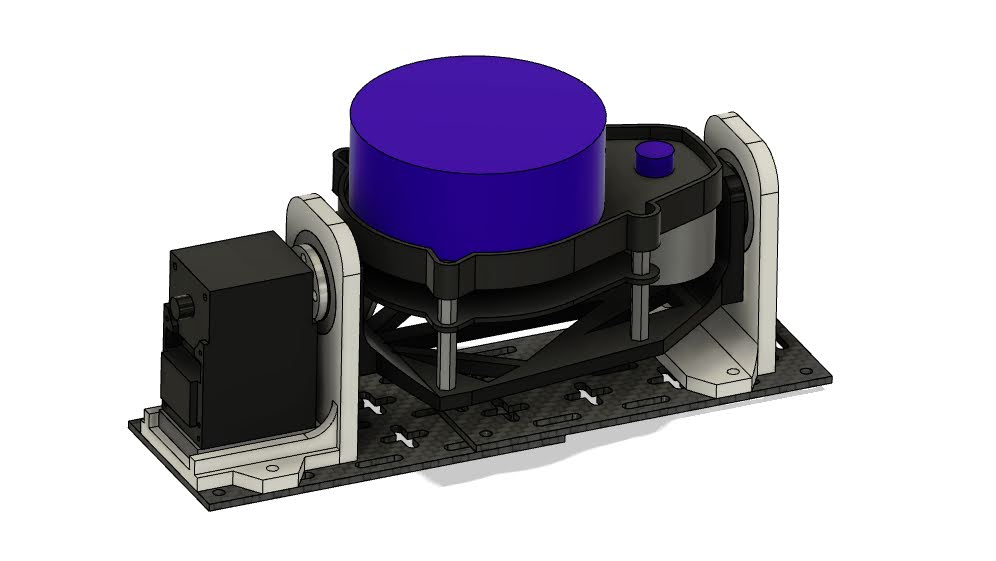
\includegraphics[width=0.7\textwidth]{design/existing_solutions/3D_3.jpg}
    \caption{Implementation in project \cite{lidar_design_3} using a tilting platform}
    \label{ph:lidar_design_3}
\end{figure}

\begin{tabular}{p{0.45\linewidth} p{0.45\linewidth}}
\textbf{Pros} & \textbf{Cons} \\
\begin{itemize}[label=\textcolor{green!60!black}{\textbf{+}}]
    \item Faster data acquisition compared to solutions with single-point \gls{lidar} measurements
    \item Higher resolution given by the use of a 2D \gls{lidar} sensor
    \item This design could be potentially used for \gls{slam} applications, given the higher speed
\end{itemize}
&
\begin{itemize}[label=\textcolor{red!70!black}{\textbf{--}}]
    \item More expensive than single-point \gls{lidar} solutions
    \item Point distribution is non-uniform due to the tilting mechanism, which produces denser point clouds on the axis of tilting (see \cref{fig:tilt_pointCloud})
    \item Mechanical design is more prone to vibrations produced by the \gls{lidar} itself, affecting measurement accuracy
\end{itemize}
\end{tabular}
\begin{figure}[H]
    \centering
    % This file was created by matlab2tikz.
%
%The latest updates can be retrieved from
%  http://www.mathworks.com/matlabcentral/fileexchange/22022-matlab2tikz-matlab2tikz
%where you can also make suggestions and rate matlab2tikz.
%
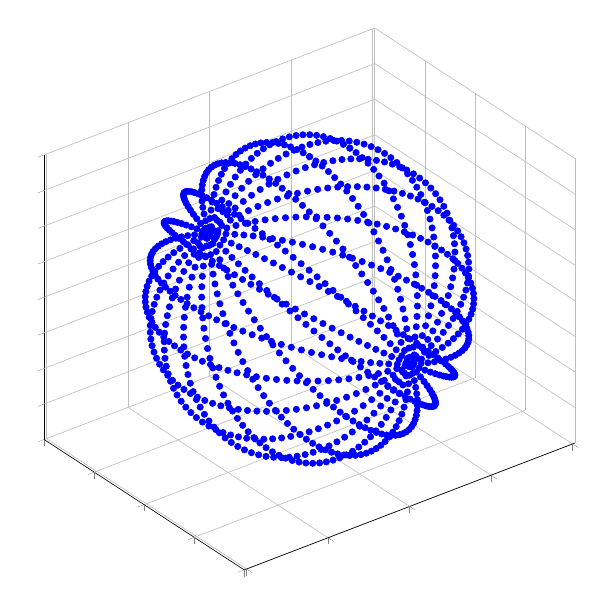
\begin{tikzpicture}[scale=0.57]

\begin{axis}[%
width=4.656in,
height=4.754in,
at={(1.697in,0.642in)},
scale only axis,
plot box ratio=1.268 1 1,
xmin=-5.07157464212679,
xmax=5.07157464212679,
xtick={-5,-2.5,0,2.5,5},
xticklabels={\empty},
tick align=outside,
ymin=-4,
ymax=4,
ytick={-4,-2,0,2,4},
yticklabels={\empty},
zmin=-3.99899308476637,
zmax=4.00100691523363,
ztick={-3,-2,-1,0,1,2,3,4},
zticklabels={\empty},
view={-37.5}{30},
axis background/.style={fill=white},
axis x line*=bottom,
axis y line*=left,
axis z line*=left,
xmajorgrids,
ymajorgrids,
zmajorgrids
]
\addplot3 [color=blue, only marks, mark=*, mark options={solid, fill=blue, blue}]
 table[row sep=crcr] {%
0	4	0\\
-0.253695678626258	3.99194670588754	0\\
-0.506369814294997	3.96781925132318	0\\
-0.757004977441641	3.92771478905083	0\\
-1.00459194872432	3.87179480558542	0\\
-1.24813378279395	3.80028447096378	0\\
-1.48664982264131	3.71347173206429	0\\
-1.71917964835669	3.61170615314649	0\\
-1.94478694440187	3.49539750827914	0\\
-2.16256326982239	3.36501413132472	0\\
-2.37163171621856	3.22108103012423	0\\
-2.57115043874616	3.06417777247591	0\\
-2.76031604592845	2.89493615242028	0\\
-2.93836683463013	2.71403764622853	0\\
-3.10458585716703	2.52221066833809	0\\
-3.25830380820134	2.32022763828479	0\\
-3.39890171979806	2.10890187044201	0\\
-3.52581345379033	1.88908429909073	0\\
-3.63852798141807	1.66166005200755	0\\
-3.73659144106043	1.42754488636749	0\\
-3.8196089657763	1.1876815013131	0\\
-3.88724627329417	0.943035742037709	0\\
-3.93923101204883	0.694592710667723	0\\
-3.97535385784502	0.443352799604044	0\\
-3.99546935673203	0.19032766329497	0\\
-3.9994965106955	-0.0634638553392321	0\\
-3.98741910380777	-0.316999827427154	0\\
-3.95928576752373	-0.56925935309314	0\\
-3.91520978485911	-0.819226672260762	0\\
-3.85536863423977	-1.06589525476014	0\\
-3.78000327485867	-1.30827185326969	0\\
-3.68941717641833	-1.54538050277251	0\\
-3.58397509716534	-1.7762664504231	0\\
-3.46410161513775	-2	0\\
-3.33027941853909	-2.21568025546444	0\\
-3.18304736212333	-2.42243874855067	0\\
-3.02299829741703	-2.61944293578114	0\\
-2.85077668551545	-2.80589955082529	0\\
-2.66707600206517	-2.98105779870302	0\\
-2.47263594488242	-3.14421237897115	0\\
-2.26823945545108	-3.29470632571933	0\\
-2.05470956629363	-3.43193365293991	0\\
-1.83290608690964	-3.55534179461969	0\\
-1.60372214162646	-3.66443382972828	0\\
-1.36808057330268	-3.75877048314363	0\\
-1.12693022736572	-3.83797189445799	0\\
-0.881242131146163	-3.90171914754163	0\\
-0.6320055838934	-3.94975555470558	0\\
-0.380224173216732	-3.98188769029234	0\\
-0.126911733992272	-3.99798616953274	0\\
0.126911733992271	-3.99798616953274	0\\
0.380224173216731	-3.98188769029234	0\\
0.6320055838934	-3.94975555470558	0\\
0.881242131146162	-3.90171914754163	0\\
1.12693022736572	-3.83797189445799	0\\
1.36808057330267	-3.75877048314363	0\\
1.60372214162645	-3.66443382972828	0\\
1.83290608690964	-3.55534179461969	0\\
2.05470956629363	-3.43193365293991	0\\
2.26823945545108	-3.29470632571933	0\\
2.47263594488242	-3.14421237897115	0\\
2.66707600206517	-2.98105779870302	0\\
2.85077668551545	-2.80589955082529	0\\
3.02299829741703	-2.61944293578114	0\\
3.18304736212333	-2.42243874855067	0\\
3.33027941853909	-2.21568025546444	0\\
3.46410161513775	-2	0\\
3.58397509716534	-1.7762664504231	0\\
3.68941717641833	-1.54538050277251	0\\
3.78000327485867	-1.30827185326969	0\\
3.85536863423977	-1.06589525476014	0\\
3.91520978485911	-0.819226672260762	0\\
3.95928576752373	-0.569259353093141	0\\
3.98741910380777	-0.316999827427155	0\\
3.9994965106955	-0.0634638553392304	0\\
3.99546935673203	0.19032766329497	0\\
3.97535385784502	0.443352799604043	0\\
3.93923101204883	0.69459271066772	0\\
3.88724627329417	0.943035742037706	0\\
3.8196089657763	1.1876815013131	0\\
3.73659144106043	1.42754488636749	0\\
3.63852798141807	1.66166005200754	0\\
3.52581345379033	1.88908429909073	0\\
3.39890171979806	2.10890187044201	0\\
3.25830380820134	2.32022763828479	0\\
3.10458585716703	2.52221066833809	0\\
2.93836683463014	2.71403764622853	0\\
2.76031604592845	2.89493615242028	0\\
2.57115043874616	3.06417777247591	0\\
2.37163171621856	3.22108103012423	0\\
2.16256326982239	3.36501413132472	0\\
1.94478694440188	3.49539750827914	0\\
1.71917964835669	3.61170615314648	0\\
1.48664982264131	3.71347173206429	0\\
1.24813378279395	3.80028447096378	0\\
1.00459194872432	3.87179480558542	0\\
0.757004977441643	3.92771478905083	0\\
0.506369814295	3.96781925132318	0\\
0.253695678626262	3.99194670588754	0\\
9.79717439317883e-16	4	0\\
};
 \addplot3 [color=blue, only marks, mark=*, mark options={solid, fill=blue, blue}]
 table[row sep=crcr] {%
0	4	0\\
-0.241278928313424	3.99194670588754	0.0783962760949988\\
-0.481586311540424	3.96781925132318	0.15647687805564\\
-0.719954516663738	3.92771478905083	0.233927402855891\\
-0.955423719051908	3.87179480558542	0.31043598456806\\
-1.1870457673343	3.80028447096378	0.385694550136819\\
-1.41388800127205	3.71347173206429	0.459400059880666\\
-1.63503700725164	3.61170615314649	0.531255727725762\\
-1.84960229627914	3.49539750827914	0.600972216258705\\
-2.05671988966514	3.36501413132472	0.668268801786173\\
-2.25555579796192	3.22108103012423	0.732874504710158\\
-2.44530937914468	3.06417777247591	0.794529180667165\\
-2.62521656251432	2.89493615242028	0.852984568037748\\
-2.79455292534055	2.71403764622853	0.908005287608432\\
-2.95263660985648	2.52221066833809	0.959369790360725\\
-3.0988310688592	2.32022763828479	1.00687124957082\\
-3.23254762886075	2.10890187044201	1.05031839362784\\
-3.35324786046841	1.88908429909073	1.08953627621704\\
-3.46044574644991	1.66166005200755	1.12436698076696\\
-3.55370963875322	1.42754488636749	1.15467025632365\\
-3.63266399660094	1.1876815013131	1.18032408229179\\
-3.69699089866047	0.943035742037709	1.20122515976858\\
-3.74643132320099	0.694592710667723	1.21728932749191\\
-3.78078619108258	0.443352799604044	1.22845190072812\\
-3.7999171673776	0.19032766329497	1.23466793173454\\
-3.80374721839669	-0.0634638553392321	1.23591239074821\\
-3.79226092187616	-0.316999827427154	1.23218026677192\\
-3.7655045290781	-0.56925935309314	1.22348658775169\\
-3.72358577855281	-0.819226672260762	1.20986636006455\\
-3.66667346231368	-1.06589525476014	1.19137442756022\\
-3.59499674617136	-1.30827185326969	1.16808525072429\\
-3.50884424696392	-1.54538050277251	1.1400926068521\\
-3.40856287039866	-1.7762664504231	1.10750921244069\\
-3.29455641418533	-2	1.07046626931927\\
-3.16728394208523	-2.21568025546444	1.0291129363457\\
-3.02725793542349	-2.42243874855067	0.983615728796456\\
-2.87504222950762	-2.61944293578114	0.934157847868395\\
-2.71124974326177	-2.80589955082529	0.880938442992159\\
-2.5365400112185	-2.98105779870302	0.824171809927729\\
-2.35161652780605	-3.14421237897115	0.764086527871024\\
-2.15722391462452	-3.29470632571933	0.700924539046161\\
-1.95414492211754	-3.43193365293991	0.634940174489508\\
-1.74319727771247	-3.55534179461969	0.566399129948364\\
-1.52523039312066	-3.66443382972828	0.495577396017961\\
-1.30112194405632	-3.75877048314363	0.422760146824748\\
-1.07177433614615	-3.83797189445799	0.34824059173083\\
-0.838111071260387	-3.90171914754163	0.272318794683361\\
-0.601073028896741	-3.94975555470558	0.195300465962922\\
-0.36161467759071	-3.98188769029234	0.117495731196134\\
-0.120700231607668	-3.99798616953274	0.0392178825892049\\
0.120700231607667	-3.99798616953274	-0.0392178825892046\\
0.361614677590709	-3.98188769029234	-0.117495731196133\\
0.601073028896742	-3.94975555470558	-0.195300465962922\\
0.838111071260386	-3.90171914754163	-0.27231879468336\\
1.07177433614614	-3.83797189445799	-0.34824059173083\\
1.30112194405632	-3.75877048314363	-0.422760146824747\\
1.52523039312066	-3.66443382972828	-0.49557739601796\\
1.74319727771246	-3.55534179461969	-0.566399129948363\\
1.95414492211754	-3.43193365293991	-0.634940174489508\\
2.15722391462452	-3.29470632571933	-0.700924539046161\\
2.35161652780605	-3.14421237897115	-0.764086527871023\\
2.5365400112185	-2.98105779870302	-0.824171809927729\\
2.71124974326177	-2.80589955082529	-0.880938442992159\\
2.87504222950762	-2.61944293578114	-0.934157847868395\\
3.02725793542349	-2.42243874855067	-0.983615728796456\\
3.16728394208523	-2.21568025546444	-1.0291129363457\\
3.29455641418533	-2	-1.07046626931927\\
3.40856287039866	-1.7762664504231	-1.10750921244069\\
3.50884424696391	-1.54538050277251	-1.1400926068521\\
3.59499674617136	-1.30827185326969	-1.16808525072429\\
3.66667346231368	-1.06589525476014	-1.19137442756022\\
3.72358577855281	-0.819226672260762	-1.20986636006455\\
3.7655045290781	-0.569259353093141	-1.22348658775169\\
3.79226092187616	-0.316999827427155	-1.23218026677192\\
3.80374721839669	-0.0634638553392304	-1.23591239074821\\
3.7999171673776	0.19032766329497	-1.23466793173454\\
3.78078619108258	0.443352799604043	-1.22845190072812\\
3.746431323201	0.69459271066772	-1.21728932749191\\
3.69699089866047	0.943035742037706	-1.20122515976858\\
3.63266399660094	1.1876815013131	-1.18032408229179\\
3.55370963875322	1.42754488636749	-1.15467025632365\\
3.46044574644991	1.66166005200754	-1.12436698076696\\
3.35324786046841	1.88908429909073	-1.08953627621704\\
3.23254762886075	2.10890187044201	-1.05031839362784\\
3.0988310688592	2.32022763828479	-1.00687124957082\\
2.95263660985648	2.52221066833809	-0.959369790360725\\
2.79455292534055	2.71403764622853	-0.908005287608432\\
2.62521656251433	2.89493615242028	-0.852984568037749\\
2.44530937914468	3.06417777247591	-0.794529180667166\\
2.25555579796192	3.22108103012423	-0.732874504710158\\
2.05671988966514	3.36501413132472	-0.668268801786173\\
1.84960229627914	3.49539750827914	-0.600972216258705\\
1.63503700725164	3.61170615314648	-0.531255727725763\\
1.41388800127205	3.71347173206429	-0.459400059880667\\
1.1870457673343	3.80028447096378	-0.385694550136819\\
0.955423719051909	3.87179480558542	-0.31043598456806\\
0.71995451666374	3.92771478905083	-0.233927402855891\\
0.481586311540426	3.96781925132318	-0.156476878055641\\
0.241278928313427	3.99194670588754	-0.078396276095\\
9.31766654791274e-16	4	-3.02749338434732e-16\\
};
 \addplot3 [color=blue, only marks, mark=*, mark options={solid, fill=blue, blue}]
 table[row sep=crcr] {%
0	4	0\\
-0.205244115408128	3.99194670588754	0.149118578466845\\
-0.409661785203139	3.96781925132318	0.297636709048678\\
-0.612429891576711	3.92771478905083	0.444956361652193\\
-0.812731958930218	3.87179480558542	0.59048433203191\\
-1.00976144153379	3.80028447096378	0.7336346304143\\
-1.20272497120132	3.71347173206429	0.873830841071783\\
-1.3908455519041	3.61170615314649	1.01050844334542\\
-1.57336568845964	3.49539750827914	1.14311708477036\\
-1.74955043669737	3.36501413132472	1.27112279715099\\
-1.91869036281944	3.22108103012423	1.39401014666236\\
-2.08010440004024	3.06417777247591	1.51128430932031\\
-2.23314259100197	2.89493615242028	1.62247306346301\\
-2.3771887049235	2.71403764622853	1.72712869122091\\
-2.51166271894424	2.52221066833809	1.82482978131856\\
-2.63602315367149	2.32022763828479	1.91518292594915\\
-2.74976925352686	2.10890187044201	1.99782430488882\\
-2.8524430031122	1.88908429909073	2.07242115047234\\
-2.94363097147599	1.66166005200755	2.13867308753104\\
-3.02296597685386	1.42754488636749	2.1963133428976\\
-3.09012856517994	1.1876815013131	2.24510981960741\\
-3.14484829641566	0.943035742037709	2.28486603147119\\
-3.18690483351633	0.694592710667723	2.31542189425546\\
-3.21612882965063	0.443352799604044	2.33665437028529\\
-3.23240261010055	0.19032766329497	2.34847796387358\\
-3.23566064609596	-0.0634638553392321	2.35084506558202\\
-3.22588981867581	-0.316999827427154	2.34374614392748\\
-3.20312947151355	-0.56925935309314	2.32720978376193\\
-3.16747125249411	-0.819226672260762	2.30130257117137\\
-3.1190587446801	-1.06589525476014	2.26612882535711\\
-3.05808688815362	-1.30827185326969	2.22183017857918\\
-2.98480119506126	-1.54538050277251	2.16858500585323\\
-2.89949676102337	-1.7762664504231	2.10660770669727\\
-2.80251707688815	-2	2.03614784182051\\
-2.69425264561524	-2.21568025546444	1.95748912823043\\
-2.57513940985812	-2.42243874855067	1.87094829680455\\
-2.44565699657691	-2.61944293578114	1.77687381692699\\
-2.30632678574988	-2.80589955082529	1.6756444933252\\
-2.15770981096031	-2.98105779870302	1.56766794075707\\
-2.00040450031223	-3.14421237897115	1.45337894269015\\
-1.8350442667717	-3.29470632571933	1.33323770058206\\
-1.66229495763632	-3.43193365293991	1.20772798081166\\
-1.48285217340318	-3.55534179461969	1.07735516672259\\
-1.29743846683119	-3.66443382972828	0.942644223622932\\
-1.10680043347609	-3.75877048314363	0.804137584935145\\
-0.91170570541369	-3.83797189445799	0.662392968008173\\
-0.712939860256442	-3.90171914754163	0.517981128386504\\
-0.511303257909622	-3.94975555470558	0.371483561579034\\
-0.307607817804499	-3.98188769029234	0.223490161581893\\
-0.102673749585341	-3.99798616953274	0.0745968455835231\\
0.10267374958534	-3.99798616953274	-0.0745968455835225\\
0.307607817804499	-3.98188769029234	-0.223490161581893\\
0.511303257909622	-3.94975555470558	-0.371483561579034\\
0.712939860256441	-3.90171914754163	-0.517981128386504\\
0.911705705413689	-3.83797189445799	-0.662392968008172\\
1.10680043347608	-3.75877048314363	-0.804137584935144\\
1.29743846683119	-3.66443382972828	-0.94264422362293\\
1.48285217340318	-3.55534179461969	-1.07735516672259\\
1.66229495763632	-3.43193365293991	-1.20772798081166\\
1.8350442667717	-3.29470632571933	-1.33323770058206\\
2.00040450031223	-3.14421237897115	-1.45337894269015\\
2.15770981096031	-2.98105779870302	-1.56766794075707\\
2.30632678574988	-2.80589955082529	-1.6756444933252\\
2.44565699657691	-2.61944293578114	-1.77687381692699\\
2.57513940985812	-2.42243874855067	-1.87094829680455\\
2.69425264561524	-2.21568025546444	-1.95748912823043\\
2.80251707688815	-2	-2.03614784182051\\
2.89949676102337	-1.7762664504231	-2.10660770669727\\
2.98480119506126	-1.54538050277251	-2.16858500585323\\
3.05808688815362	-1.30827185326969	-2.22183017857918\\
3.1190587446801	-1.06589525476014	-2.26612882535711\\
3.16747125249411	-0.819226672260762	-2.30130257117137\\
3.20312947151355	-0.569259353093141	-2.32720978376193\\
3.22588981867581	-0.316999827427155	-2.34374614392748\\
3.23566064609596	-0.0634638553392304	-2.35084506558202\\
3.23240261010055	0.19032766329497	-2.34847796387358\\
3.21612882965063	0.443352799604043	-2.33665437028529\\
3.18690483351633	0.69459271066772	-2.31542189425546\\
3.14484829641566	0.943035742037706	-2.28486603147119\\
3.09012856517994	1.1876815013131	-2.24510981960741\\
3.02296597685386	1.42754488636749	-2.1963133428976\\
2.94363097147599	1.66166005200754	-2.13867308753105\\
2.8524430031122	1.88908429909073	-2.07242115047234\\
2.74976925352686	2.10890187044201	-1.99782430488882\\
2.6360231536715	2.32022763828479	-1.91518292594915\\
2.51166271894424	2.52221066833809	-1.82482978131857\\
2.3771887049235	2.71403764622853	-1.72712869122091\\
2.23314259100197	2.89493615242028	-1.62247306346302\\
2.08010440004025	3.06417777247591	-1.51128430932031\\
1.91869036281944	3.22108103012423	-1.39401014666236\\
1.74955043669737	3.36501413132472	-1.27112279715099\\
1.57336568845964	3.49539750827914	-1.14311708477036\\
1.39084555190411	3.61170615314648	-1.01050844334542\\
1.20272497120132	3.71347173206429	-0.873830841071784\\
1.00976144153379	3.80028447096378	-0.7336346304143\\
0.812731958930219	3.87179480558542	-0.59048433203191\\
0.612429891576712	3.92771478905083	-0.444956361652194\\
0.409661785203141	3.96781925132318	-0.297636709048679\\
0.205244115408131	3.99194670588754	-0.149118578466847\\
7.92608058093673e-16	4	-5.75863462244797e-16\\
};
 \addplot3 [color=blue, only marks, mark=*, mark options={solid, fill=blue, blue}]
 table[row sep=crcr] {%
0	4	0\\
-0.149118578466845	3.99194670588754	0.205244115408128\\
-0.297636709048678	3.96781925132318	0.409661785203139\\
-0.444956361652193	3.92771478905083	0.612429891576711\\
-0.59048433203191	3.87179480558542	0.812731958930218\\
-0.7336346304143	3.80028447096378	1.00976144153379\\
-0.873830841071783	3.71347173206429	1.20272497120132\\
-1.01050844334542	3.61170615314649	1.3908455519041\\
-1.14311708477036	3.49539750827914	1.57336568845964\\
-1.27112279715099	3.36501413132472	1.74955043669737\\
-1.39401014666236	3.22108103012423	1.91869036281944\\
-1.51128430932031	3.06417777247591	2.08010440004024\\
-1.62247306346301	2.89493615242028	2.23314259100197\\
-1.72712869122091	2.71403764622853	2.3771887049235\\
-1.82482978131857	2.52221066833809	2.51166271894424\\
-1.91518292594915	2.32022763828479	2.63602315367149\\
-1.99782430488882	2.10890187044201	2.74976925352686\\
-2.07242115047234	1.88908429909073	2.8524430031122\\
-2.13867308753105	1.66166005200755	2.94363097147599\\
-2.1963133428976	1.42754488636749	3.02296597685386\\
-2.24510981960741	1.1876815013131	3.09012856517994\\
-2.28486603147119	0.943035742037709	3.14484829641566\\
-2.31542189425546	0.694592710667723	3.18690483351633\\
-2.33665437028529	0.443352799604044	3.21612882965063\\
-2.34847796387358	0.19032766329497	3.23240261010055\\
-2.35084506558202	-0.0634638553392321	3.23566064609596\\
-2.34374614392748	-0.316999827427154	3.22588981867581\\
-2.32720978376193	-0.56925935309314	3.20312947151355\\
-2.30130257117137	-0.819226672260762	3.16747125249411\\
-2.26612882535711	-1.06589525476014	3.1190587446801\\
-2.22183017857918	-1.30827185326969	3.05808688815362\\
-2.16858500585323	-1.54538050277251	2.98480119506126\\
-2.10660770669727	-1.7762664504231	2.89949676102337\\
-2.03614784182051	-2	2.80251707688815\\
-1.95748912823043	-2.21568025546444	2.69425264561524\\
-1.87094829680455	-2.42243874855067	2.57513940985812\\
-1.77687381692699	-2.61944293578114	2.44565699657691\\
-1.6756444933252	-2.80589955082529	2.30632678574988\\
-1.56766794075707	-2.98105779870302	2.15770981096031\\
-1.45337894269015	-3.14421237897115	2.00040450031223\\
-1.33323770058206	-3.29470632571933	1.8350442667717\\
-1.20772798081166	-3.43193365293991	1.66229495763632\\
-1.07735516672259	-3.55534179461969	1.48285217340318\\
-0.942644223622932	-3.66443382972828	1.29743846683119\\
-0.804137584935145	-3.75877048314363	1.10680043347609\\
-0.662392968008173	-3.83797189445799	0.91170570541369\\
-0.517981128386504	-3.90171914754163	0.712939860256442\\
-0.371483561579034	-3.94975555470558	0.511303257909622\\
-0.223490161581894	-3.98188769029234	0.307607817804499\\
-0.0745968455835231	-3.99798616953274	0.102673749585341\\
0.0745968455835225	-3.99798616953274	-0.10267374958534\\
0.223490161581893	-3.98188769029234	-0.307607817804499\\
0.371483561579034	-3.94975555470558	-0.511303257909622\\
0.517981128386504	-3.90171914754163	-0.712939860256441\\
0.662392968008172	-3.83797189445799	-0.911705705413689\\
0.804137584935144	-3.75877048314363	-1.10680043347608\\
0.94264422362293	-3.66443382972828	-1.29743846683119\\
1.07735516672259	-3.55534179461969	-1.48285217340318\\
1.20772798081166	-3.43193365293991	-1.66229495763632\\
1.33323770058206	-3.29470632571933	-1.8350442667717\\
1.45337894269015	-3.14421237897115	-2.00040450031223\\
1.56766794075707	-2.98105779870302	-2.15770981096031\\
1.6756444933252	-2.80589955082529	-2.30632678574988\\
1.77687381692699	-2.61944293578114	-2.44565699657691\\
1.87094829680455	-2.42243874855067	-2.57513940985812\\
1.95748912823043	-2.21568025546444	-2.69425264561524\\
2.03614784182051	-2	-2.80251707688815\\
2.10660770669727	-1.7762664504231	-2.89949676102337\\
2.16858500585323	-1.54538050277251	-2.98480119506126\\
2.22183017857918	-1.30827185326969	-3.05808688815362\\
2.26612882535711	-1.06589525476014	-3.1190587446801\\
2.30130257117137	-0.819226672260762	-3.16747125249411\\
2.32720978376193	-0.569259353093141	-3.20312947151355\\
2.34374614392748	-0.316999827427155	-3.22588981867581\\
2.35084506558202	-0.0634638553392304	-3.23566064609596\\
2.34847796387358	0.19032766329497	-3.23240261010055\\
2.33665437028529	0.443352799604043	-3.21612882965063\\
2.31542189425546	0.69459271066772	-3.18690483351633\\
2.28486603147119	0.943035742037706	-3.14484829641566\\
2.24510981960741	1.1876815013131	-3.09012856517994\\
2.1963133428976	1.42754488636749	-3.02296597685386\\
2.13867308753105	1.66166005200754	-2.94363097147599\\
2.07242115047235	1.88908429909073	-2.8524430031122\\
1.99782430488882	2.10890187044201	-2.74976925352686\\
1.91518292594915	2.32022763828479	-2.6360231536715\\
1.82482978131857	2.52221066833809	-2.51166271894424\\
1.72712869122091	2.71403764622853	-2.3771887049235\\
1.62247306346302	2.89493615242028	-2.23314259100197\\
1.51128430932032	3.06417777247591	-2.08010440004025\\
1.39401014666236	3.22108103012423	-1.91869036281944\\
1.27112279715099	3.36501413132472	-1.74955043669737\\
1.14311708477036	3.49539750827914	-1.57336568845964\\
1.01050844334542	3.61170615314648	-1.39084555190411\\
0.873830841071784	3.71347173206429	-1.20272497120132\\
0.7336346304143	3.80028447096378	-1.00976144153379\\
0.59048433203191	3.87179480558542	-0.812731958930219\\
0.444956361652194	3.92771478905083	-0.612429891576712\\
0.297636709048679	3.96781925132318	-0.409661785203141\\
0.149118578466847	3.99194670588754	-0.205244115408131\\
5.75863462244797e-16	4	-7.92608058093673e-16\\
};
 \addplot3 [color=blue, only marks, mark=*, mark options={solid, fill=blue, blue}]
 table[row sep=crcr] {%
-1.23606797749979	0	3.80422606518061\\
-1.23357937275834	-0.253695678626258	3.79656692733732\\
-1.22612357926694	-0.506369814294997	3.77362035445227\\
-1.21373061887452	-0.757004977441641	3.73547874427563\\
-1.19645039365854	-1.00459194872432	3.68229567960975\\
-1.17435248498702	-1.24813378279395	3.61428530988539\\
-1.14752587333884	-1.48664982264131	3.53172148885759\\
-1.11607858001083	-1.71917964835669	3.43493667189327\\
-1.0801372321541	-1.94478694440188	3.32432057729072\\
-1.03984655289119	-2.16256326982239	3.20031861702166\\
-0.995368778567151	-2.37163171621856	3.06343010321436\\
-0.946883005481028	-2.57115043874616	2.91420623759999\\
-0.89458446872829	-2.76031604592845	2.75324789201773\\
-0.838683756057997	-2.93836683463013	2.581203188916\\
-0.779405959910264	-3.10458585716703	2.3987648915921\\
-0.71698977104845	-3.25830380820134	2.20666761467887\\
-0.651686517435695	-3.39890171979806	2.00568486611091\\
-0.583759152225922	-3.52581345379033	1.7966259324811\\
-0.513481194944291	-3.63852798141807	1.58033262032912\\
-0.441135630120607	-3.73659144106043	1.35767586648362\\
-0.367013767810499	-3.8196089657763	1.12955223110703\\
-0.291414070592641	-3.88724627329417	0.896880287564199\\
-0.214640951765287	-3.93923101204883	0.660596923651652\\
-0.13700354958136	-3.97535385784502	0.421653569081126\\
-0.0588144824578185	-3.99546935673203	0.181012364407911\\
0.019611409828376	-3.9994965106955	-0.0603577131695897\\
0.0979583338889162	-3.98741910380777	-0.301484751539034\\
0.175910814312669	-3.95928576752373	-0.541397817221195\\
0.253154963973811	-3.91520978485912	-0.779130864976392\\
0.329379747944498	-3.85536863423977	-1.01372662772771\\
0.404278235922741	-3.78000327485868	-1.24424047113767\\
0.477548838132408	-3.68941717641833	-1.46974419731728\\
0.548896519718802	-3.58397509716534	-1.68932978235135\\
0.618033988749895	-3.46410161513776	-1.90211303259031\\
0.684682853039538	-3.33027941853909	-2.10723714498597\\
0.748574741134536	-3.18304736212333	-2.30387615713499\\
0.809452382951777	-3.02299829741703	-2.49123827313796\\
0.867070645714045	-2.85077668551545	-2.66856905188203\\
0.921197521013204	-2.66707600206517	-2.83515444490899\\
0.971615059026168	-2.47263594488242	-2.9903236716364\\
1.01812024612191	-2.26823945545108	-3.13345192035423\\
1.06052582232572	-2.05470956629363	-3.26396286412113\\
1.09866103534901	-1.83290608690964	-3.38133098142957\\
1.13237232814851	-1.60372214162646	-3.48508367229548\\
1.16152395724631	-1.36808057330268	-3.57480316125163\\
1.18599853932093	-1.12693022736572	-3.65012817958193\\
1.2056975238685	-0.881242131146163	-3.71075542002304\\
1.22054159003087	-0.6320055838934	-3.75644075807572\\
1.23047096599274	-0.380224173216732	-3.78700023500799\\
1.23544566966162	-0.126911733992272	-3.80231079859201\\
1.23544566966162	0.126911733992271	-3.80231079859201\\
1.23047096599274	0.380224173216731	-3.78700023500799\\
1.22054159003087	0.6320055838934	-3.75644075807572\\
1.2056975238685	0.881242131146162	-3.71075542002304\\
1.18599853932093	1.12693022736572	-3.65012817958193\\
1.16152395724632	1.36808057330267	-3.57480316125164\\
1.13237232814851	1.60372214162645	-3.48508367229548\\
1.09866103534901	1.83290608690964	-3.38133098142957\\
1.06052582232572	2.05470956629363	-3.26396286412113\\
1.01812024612191	2.26823945545108	-3.13345192035423\\
0.971615059026169	2.47263594488242	-2.9903236716364\\
0.921197521013204	2.66707600206517	-2.83515444490899\\
0.867070645714045	2.85077668551545	-2.66856905188203\\
0.809452382951777	3.02299829741703	-2.49123827313796\\
0.748574741134536	3.18304736212333	-2.30387615713499\\
0.684682853039538	3.33027941853909	-2.10723714498597\\
0.618033988749896	3.46410161513775	-1.90211303259031\\
0.548896519718802	3.58397509716534	-1.68932978235135\\
0.477548838132408	3.68941717641833	-1.46974419731728\\
0.404278235922741	3.78000327485867	-1.24424047113767\\
0.329379747944498	3.85536863423977	-1.01372662772772\\
0.253154963973811	3.91520978485912	-0.779130864976392\\
0.175910814312669	3.95928576752373	-0.541397817221195\\
0.0979583338889165	3.98741910380777	-0.301484751539035\\
0.0196114098283755	3.9994965106955	-0.0603577131695881\\
-0.0588144824578185	3.99546935673203	0.181012364407911\\
-0.13700354958136	3.97535385784502	0.421653569081125\\
-0.214640951765286	3.93923101204883	0.660596923651649\\
-0.29141407059264	3.88724627329417	0.896880287564196\\
-0.367013767810499	3.8196089657763	1.12955223110703\\
-0.441135630120607	3.73659144106043	1.35767586648362\\
-0.51348119494429	3.63852798141808	1.58033262032912\\
-0.583759152225921	3.52581345379033	1.7966259324811\\
-0.651686517435695	3.39890171979806	2.00568486611091\\
-0.716989771048449	3.25830380820134	2.20666761467887\\
-0.779405959910264	3.10458585716703	2.39876489159209\\
-0.838683756057996	2.93836683463014	2.581203188916\\
-0.894584468728289	2.76031604592845	2.75324789201773\\
-0.946883005481027	2.57115043874616	2.91420623759998\\
-0.995368778567151	2.37163171621856	3.06343010321436\\
-1.03984655289119	2.16256326982239	3.20031861702166\\
-1.0801372321541	1.94478694440188	3.32432057729072\\
-1.11607858001083	1.71917964835669	3.43493667189327\\
-1.14752587333884	1.48664982264131	3.53172148885759\\
-1.17435248498702	1.24813378279395	3.61428530988539\\
-1.19645039365854	1.00459194872432	3.68229567960975\\
-1.21373061887452	0.757004977441643	3.73547874427563\\
-1.22612357926694	0.506369814295	3.77362035445227\\
-1.23357937275834	0.253695678626262	3.79656692733732\\
-1.23606797749979	9.79717439317883e-16	3.80422606518061\\
};
 \addplot3 [color=blue, only marks, mark=*, mark options={solid, fill=blue, blue}]
 table[row sep=crcr] {%
-4.89858719658941e-16	0	4\\
-4.88872475573199e-16	-0.253695678626258	3.99194670588754\\
-4.85917714572818e-16	-0.506369814294997	3.96781925132318\\
-4.81006334437482e-16	-0.757004977441641	3.92771478905083\\
-4.74158111561554e-16	-1.00459194872432	3.87179480558542\\
-4.65400621321519e-16	-1.24813378279395	3.80028447096378\\
-4.54769127039671e-16	-1.48664982264131	3.71347173206429\\
-4.42306437991164e-16	-1.71917964835669	3.61170615314649\\
-4.28062737026168e-16	-1.94478694440187	3.49539750827914\\
-4.12095378501244e-16	-2.16256326982239	3.36501413132472\\
-3.9446865733359e-16	-2.37163171621856	3.22108103012423\\
-3.75253550108109e-16	-2.57115043874616	3.06417777247591\\
-3.54527429279745e-16	-2.76031604592845	2.89493615242028\\
-3.32373751621918e-16	-2.93836683463013	2.71403764622853\\
-3.08881722175555e-16	-3.10458585716703	2.52221066833809\\
-2.84145935051869e-16	-3.25830380820134	2.32022763828479\\
-2.58265992535267e-16	-3.39890171979806	2.10890187044201\\
-2.31346104020098e-16	-3.52581345379033	1.88908429909073\\
-2.03494666396207e-16	-3.63852798141807	1.66166005200755\\
-1.74823827572912e-16	-3.73659144106043	1.42754488636749\\
-1.45449034898961e-16	-3.8196089657763	1.1876815013131\\
-1.15488570296803e-16	-3.88724627329417	0.943035742037709\\
-8.5063073983031e-17	-3.93923101204883	0.694592710667723\\
-5.42950586928111e-17	-3.97535385784502	0.443352799604044\\
-2.3308416364338e-17	-3.99546935673203	0.19032766329497\\
7.77208073027413e-18	-3.9994965106955	-0.0634638553392321\\
3.88212823988928e-17	-3.98741910380777	-0.316999827427154\\
6.97141644650207e-17	-3.95928576752373	-0.56925935309314\\
1.00326332196028e-16	-3.91520978485911	-0.819226672260762\\
1.30534521196836e-16	-3.85536863423977	-1.06589525476014\\
1.6021709375213e-16	-3.78000327485867	-1.30827185326969\\
1.89254528618509e-16	-3.68941717641833	-1.54538050277251\\
2.17529902294348e-16	-3.58397509716534	-1.7762664504231\\
2.44929359829471e-16	-3.46410161513775	-2\\
2.71342573278852e-16	-3.33027941853909	-2.21568025546444\\
2.96663185954309e-16	-3.18304736212333	-2.42243874855067\\
3.20789240685352e-16	-3.02299829741703	-2.61944293578114\\
3.43623590364718e-16	-2.85077668551545	-2.80589955082529\\
3.65074289125491e-16	-2.66707600206517	-2.98105779870302\\
3.8505496257465e-16	-2.47263594488242	-3.14421237897115\\
4.03485155592272e-16	-2.26823945545108	-3.29470632571933\\
4.20290656295894e-16	-2.05470956629363	-3.43193365293991\\
4.35403794865581e-16	-1.83290608690964	-3.55534179461969\\
4.48763716026401e-16	-1.60372214162646	-3.66443382972828\\
4.6031662409114e-16	-1.36808057330268	-3.75877048314363\\
4.70015999576548e-16	-1.12693022736572	-3.83797189445799\\
4.77822786520879e-16	-0.881242131146163	-3.90171914754163\\
4.83705549748466e-16	-0.6320055838934	-3.94975555470558\\
4.87640601448076e-16	-0.380224173216732	-3.98188769029234\\
4.89612096555366e-16	-0.126911733992272	-3.99798616953274\\
4.89612096555366e-16	0.126911733992271	-3.99798616953274\\
4.87640601448076e-16	0.380224173216731	-3.98188769029234\\
4.83705549748466e-16	0.6320055838934	-3.94975555470558\\
4.77822786520879e-16	0.881242131146162	-3.90171914754163\\
4.70015999576548e-16	1.12693022736572	-3.83797189445799\\
4.6031662409114e-16	1.36808057330267	-3.75877048314363\\
4.48763716026401e-16	1.60372214162645	-3.66443382972828\\
4.35403794865582e-16	1.83290608690964	-3.55534179461969\\
4.20290656295894e-16	2.05470956629363	-3.43193365293991\\
4.03485155592272e-16	2.26823945545108	-3.29470632571933\\
3.8505496257465e-16	2.47263594488242	-3.14421237897115\\
3.65074289125491e-16	2.66707600206517	-2.98105779870302\\
3.43623590364718e-16	2.85077668551545	-2.80589955082529\\
3.20789240685352e-16	3.02299829741703	-2.61944293578114\\
2.96663185954309e-16	3.18304736212333	-2.42243874855067\\
2.71342573278852e-16	3.33027941853909	-2.21568025546444\\
2.44929359829471e-16	3.46410161513775	-2\\
2.17529902294348e-16	3.58397509716534	-1.7762664504231\\
1.89254528618509e-16	3.68941717641833	-1.54538050277251\\
1.6021709375213e-16	3.78000327485867	-1.30827185326969\\
1.30534521196836e-16	3.85536863423977	-1.06589525476014\\
1.00326332196028e-16	3.91520978485911	-0.819226672260762\\
6.97141644650208e-17	3.95928576752373	-0.569259353093141\\
3.88212823988929e-17	3.98741910380777	-0.316999827427155\\
7.77208073027392e-18	3.9994965106955	-0.0634638553392304\\
-2.3308416364338e-17	3.99546935673203	0.19032766329497\\
-5.4295058692811e-17	3.97535385784502	0.443352799604043\\
-8.50630739830307e-17	3.93923101204883	0.69459271066772\\
-1.15488570296803e-16	3.88724627329417	0.943035742037706\\
-1.45449034898961e-16	3.8196089657763	1.1876815013131\\
-1.74823827572911e-16	3.73659144106043	1.42754488636749\\
-2.03494666396206e-16	3.63852798141807	1.66166005200754\\
-2.31346104020098e-16	3.52581345379033	1.88908429909073\\
-2.58265992535267e-16	3.39890171979806	2.10890187044201\\
-2.84145935051869e-16	3.25830380820134	2.32022763828479\\
-3.08881722175555e-16	3.10458585716703	2.52221066833809\\
-3.32373751621918e-16	2.93836683463014	2.71403764622853\\
-3.54527429279745e-16	2.76031604592845	2.89493615242028\\
-3.75253550108109e-16	2.57115043874616	3.06417777247591\\
-3.9446865733359e-16	2.37163171621856	3.22108103012423\\
-4.12095378501244e-16	2.16256326982239	3.36501413132472\\
-4.28062737026168e-16	1.94478694440188	3.49539750827914\\
-4.42306437991164e-16	1.71917964835669	3.61170615314648\\
-4.54769127039671e-16	1.48664982264131	3.71347173206429\\
-4.65400621321519e-16	1.24813378279395	3.80028447096378\\
-4.74158111561554e-16	1.00459194872432	3.87179480558542\\
-4.81006334437482e-16	0.757004977441643	3.92771478905083\\
-4.85917714572818e-16	0.506369814295	3.96781925132318\\
-4.88872475573199e-16	0.253695678626262	3.99194670588754\\
-4.89858719658941e-16	9.79717439317883e-16	4\\
};
 \addplot3 [color=blue, only marks, mark=*, mark options={solid, fill=blue, blue}]
 table[row sep=crcr] {%
1.23606797749979	0	3.80422606518061\\
1.23357937275834	-0.253695678626258	3.79656692733732\\
1.22612357926694	-0.506369814294997	3.77362035445227\\
1.21373061887452	-0.757004977441641	3.73547874427563\\
1.19645039365854	-1.00459194872432	3.68229567960975\\
1.17435248498701	-1.24813378279395	3.61428530988539\\
1.14752587333884	-1.48664982264131	3.53172148885759\\
1.11607858001083	-1.71917964835669	3.43493667189327\\
1.0801372321541	-1.94478694440187	3.32432057729072\\
1.03984655289119	-2.16256326982239	3.20031861702166\\
0.99536877856715	-2.37163171621856	3.06343010321436\\
0.946883005481028	-2.57115043874616	2.91420623759999\\
0.894584468728289	-2.76031604592845	2.75324789201773\\
0.838683756057996	-2.93836683463013	2.581203188916\\
0.779405959910264	-3.10458585716703	2.3987648915921\\
0.716989771048449	-3.25830380820134	2.20666761467887\\
0.651686517435694	-3.39890171979806	2.00568486611091\\
0.583759152225922	-3.52581345379033	1.7966259324811\\
0.51348119494429	-3.63852798141807	1.58033262032912\\
0.441135630120607	-3.73659144106043	1.35767586648362\\
0.367013767810499	-3.8196089657763	1.12955223110703\\
0.291414070592641	-3.88724627329417	0.896880287564199\\
0.214640951765287	-3.93923101204883	0.660596923651652\\
0.13700354958136	-3.97535385784502	0.421653569081126\\
0.0588144824578185	-3.99546935673203	0.181012364407911\\
-0.019611409828376	-3.9994965106955	-0.0603577131695897\\
-0.0979583338889162	-3.98741910380777	-0.301484751539034\\
-0.175910814312669	-3.95928576752373	-0.541397817221195\\
-0.253154963973811	-3.91520978485911	-0.779130864976392\\
-0.329379747944497	-3.85536863423977	-1.01372662772771\\
-0.40427823592274	-3.78000327485867	-1.24424047113767\\
-0.477548838132407	-3.68941717641833	-1.46974419731728\\
-0.548896519718802	-3.58397509716534	-1.68932978235135\\
-0.618033988749894	-3.46410161513775	-1.90211303259031\\
-0.684682853039537	-3.33027941853909	-2.10723714498597\\
-0.748574741134535	-3.18304736212333	-2.30387615713499\\
-0.809452382951776	-3.02299829741703	-2.49123827313796\\
-0.867070645714044	-2.85077668551545	-2.66856905188203\\
-0.921197521013204	-2.66707600206517	-2.83515444490899\\
-0.971615059026167	-2.47263594488242	-2.9903236716364\\
-1.01812024612191	-2.26823945545108	-3.13345192035423\\
-1.06052582232572	-2.05470956629363	-3.26396286412113\\
-1.09866103534901	-1.83290608690964	-3.38133098142957\\
-1.13237232814851	-1.60372214162646	-3.48508367229548\\
-1.16152395724631	-1.36808057330268	-3.57480316125163\\
-1.18599853932093	-1.12693022736572	-3.65012817958193\\
-1.2056975238685	-0.881242131146163	-3.71075542002304\\
-1.22054159003087	-0.6320055838934	-3.75644075807572\\
-1.23047096599274	-0.380224173216732	-3.78700023500799\\
-1.23544566966162	-0.126911733992272	-3.80231079859201\\
-1.23544566966162	0.126911733992271	-3.80231079859201\\
-1.23047096599274	0.380224173216731	-3.78700023500799\\
-1.22054159003087	0.6320055838934	-3.75644075807572\\
-1.2056975238685	0.881242131146162	-3.71075542002304\\
-1.18599853932093	1.12693022736572	-3.65012817958193\\
-1.16152395724631	1.36808057330267	-3.57480316125164\\
-1.13237232814851	1.60372214162645	-3.48508367229548\\
-1.09866103534901	1.83290608690964	-3.38133098142957\\
-1.06052582232572	2.05470956629363	-3.26396286412113\\
-1.01812024612191	2.26823945545108	-3.13345192035423\\
-0.971615059026168	2.47263594488242	-2.9903236716364\\
-0.921197521013204	2.66707600206517	-2.83515444490899\\
-0.867070645714045	2.85077668551545	-2.66856905188203\\
-0.809452382951776	3.02299829741703	-2.49123827313796\\
-0.748574741134536	3.18304736212333	-2.30387615713499\\
-0.684682853039537	3.33027941853909	-2.10723714498597\\
-0.618033988749895	3.46410161513775	-1.90211303259031\\
-0.548896519718801	3.58397509716534	-1.68932978235135\\
-0.477548838132407	3.68941717641833	-1.46974419731728\\
-0.404278235922741	3.78000327485867	-1.24424047113767\\
-0.329379747944498	3.85536863423977	-1.01372662772772\\
-0.253154963973811	3.91520978485911	-0.779130864976392\\
-0.175910814312669	3.95928576752373	-0.541397817221195\\
-0.0979583338889165	3.98741910380777	-0.301484751539035\\
-0.0196114098283754	3.9994965106955	-0.0603577131695881\\
0.0588144824578185	3.99546935673203	0.181012364407911\\
0.13700354958136	3.97535385784502	0.421653569081125\\
0.214640951765286	3.93923101204883	0.660596923651649\\
0.29141407059264	3.88724627329417	0.896880287564196\\
0.367013767810499	3.8196089657763	1.12955223110703\\
0.441135630120606	3.73659144106043	1.35767586648362\\
0.51348119494429	3.63852798141807	1.58033262032912\\
0.583759152225921	3.52581345379033	1.7966259324811\\
0.651686517435694	3.39890171979806	2.00568486611091\\
0.716989771048449	3.25830380820134	2.20666761467887\\
0.779405959910263	3.10458585716703	2.39876489159209\\
0.838683756057996	2.93836683463014	2.581203188916\\
0.894584468728288	2.76031604592845	2.75324789201773\\
0.946883005481026	2.57115043874616	2.91420623759998\\
0.99536877856715	2.37163171621856	3.06343010321436\\
1.03984655289119	2.16256326982239	3.20031861702166\\
1.0801372321541	1.94478694440188	3.32432057729072\\
1.11607858001083	1.71917964835669	3.43493667189327\\
1.14752587333884	1.48664982264131	3.53172148885759\\
1.17435248498701	1.24813378279395	3.61428530988539\\
1.19645039365854	1.00459194872432	3.68229567960975\\
1.21373061887452	0.757004977441643	3.73547874427563\\
1.22612357926694	0.506369814295	3.77362035445227\\
1.23357937275834	0.253695678626262	3.79656692733732\\
1.23606797749979	9.79717439317883e-16	3.80422606518061\\
};
 \addplot3 [color=blue, only marks, mark=*, mark options={solid, fill=blue, blue}]
 table[row sep=crcr] {%
0	-4	0\\
-0.149118578466845	-3.99194670588754	-0.205244115408128\\
-0.297636709048678	-3.96781925132318	-0.409661785203139\\
-0.444956361652193	-3.92771478905083	-0.612429891576711\\
-0.59048433203191	-3.87179480558542	-0.812731958930218\\
-0.7336346304143	-3.80028447096378	-1.00976144153379\\
-0.873830841071783	-3.71347173206429	-1.20272497120132\\
-1.01050844334542	-3.61170615314649	-1.39084555190411\\
-1.14311708477036	-3.49539750827914	-1.57336568845964\\
-1.27112279715099	-3.36501413132472	-1.74955043669737\\
-1.39401014666236	-3.22108103012423	-1.91869036281944\\
-1.51128430932031	-3.06417777247591	-2.08010440004024\\
-1.62247306346301	-2.89493615242028	-2.23314259100197\\
-1.72712869122091	-2.71403764622853	-2.3771887049235\\
-1.82482978131857	-2.52221066833809	-2.51166271894424\\
-1.91518292594915	-2.32022763828479	-2.6360231536715\\
-1.99782430488882	-2.10890187044201	-2.74976925352686\\
-2.07242115047234	-1.88908429909073	-2.8524430031122\\
-2.13867308753105	-1.66166005200755	-2.94363097147599\\
-2.1963133428976	-1.42754488636749	-3.02296597685386\\
-2.24510981960741	-1.1876815013131	-3.09012856517994\\
-2.28486603147119	-0.943035742037709	-3.14484829641566\\
-2.31542189425546	-0.694592710667723	-3.18690483351633\\
-2.33665437028529	-0.443352799604044	-3.21612882965063\\
-2.34847796387358	-0.19032766329497	-3.23240261010055\\
-2.35084506558202	0.0634638553392321	-3.23566064609596\\
-2.34374614392748	0.316999827427154	-3.22588981867581\\
-2.32720978376193	0.56925935309314	-3.20312947151356\\
-2.30130257117137	0.819226672260762	-3.16747125249411\\
-2.26612882535711	1.06589525476014	-3.1190587446801\\
-2.22183017857918	1.30827185326969	-3.05808688815362\\
-2.16858500585323	1.54538050277251	-2.98480119506126\\
-2.10660770669727	1.7762664504231	-2.89949676102337\\
-2.03614784182051	2	-2.80251707688815\\
-1.95748912823043	2.21568025546444	-2.69425264561524\\
-1.87094829680455	2.42243874855067	-2.57513940985812\\
-1.77687381692699	2.61944293578114	-2.44565699657691\\
-1.6756444933252	2.80589955082529	-2.30632678574989\\
-1.56766794075707	2.98105779870302	-2.15770981096031\\
-1.45337894269015	3.14421237897115	-2.00040450031224\\
-1.33323770058206	3.29470632571933	-1.8350442667717\\
-1.20772798081166	3.43193365293991	-1.66229495763632\\
-1.07735516672259	3.55534179461969	-1.48285217340318\\
-0.942644223622932	3.66443382972828	-1.29743846683119\\
-0.804137584935145	3.75877048314363	-1.10680043347609\\
-0.662392968008173	3.83797189445799	-0.91170570541369\\
-0.517981128386504	3.90171914754163	-0.712939860256442\\
-0.371483561579034	3.94975555470558	-0.511303257909622\\
-0.223490161581894	3.98188769029234	-0.3076078178045\\
-0.0745968455835231	3.99798616953274	-0.102673749585341\\
0.0745968455835225	3.99798616953274	0.10267374958534\\
0.223490161581893	3.98188769029234	0.307607817804499\\
0.371483561579034	3.94975555470558	0.511303257909622\\
0.517981128386504	3.90171914754163	0.712939860256442\\
0.662392968008172	3.83797189445799	0.911705705413689\\
0.804137584935144	3.75877048314363	1.10680043347609\\
0.94264422362293	3.66443382972828	1.29743846683119\\
1.07735516672259	3.55534179461969	1.48285217340318\\
1.20772798081166	3.43193365293991	1.66229495763632\\
1.33323770058206	3.29470632571933	1.8350442667717\\
1.45337894269015	3.14421237897115	2.00040450031223\\
1.56766794075707	2.98105779870302	2.15770981096031\\
1.6756444933252	2.80589955082529	2.30632678574988\\
1.77687381692699	2.61944293578114	2.44565699657691\\
1.87094829680455	2.42243874855067	2.57513940985812\\
1.95748912823043	2.21568025546444	2.69425264561524\\
2.03614784182051	2	2.80251707688815\\
2.10660770669727	1.7762664504231	2.89949676102337\\
2.16858500585323	1.54538050277251	2.98480119506126\\
2.22183017857918	1.30827185326969	3.05808688815362\\
2.26612882535711	1.06589525476014	3.1190587446801\\
2.30130257117137	0.819226672260762	3.16747125249411\\
2.32720978376193	0.569259353093141	3.20312947151356\\
2.34374614392748	0.316999827427155	3.22588981867581\\
2.35084506558202	0.0634638553392304	3.23566064609596\\
2.34847796387358	-0.19032766329497	3.23240261010055\\
2.33665437028529	-0.443352799604043	3.21612882965063\\
2.31542189425546	-0.69459271066772	3.18690483351633\\
2.28486603147119	-0.943035742037706	3.14484829641566\\
2.24510981960741	-1.1876815013131	3.09012856517994\\
2.1963133428976	-1.42754488636749	3.02296597685386\\
2.13867308753105	-1.66166005200754	2.943630971476\\
2.07242115047235	-1.88908429909073	2.85244300311221\\
1.99782430488882	-2.10890187044201	2.74976925352686\\
1.91518292594915	-2.32022763828479	2.6360231536715\\
1.82482978131857	-2.52221066833809	2.51166271894424\\
1.72712869122091	-2.71403764622853	2.3771887049235\\
1.62247306346302	-2.89493615242028	2.23314259100197\\
1.51128430932032	-3.06417777247591	2.08010440004025\\
1.39401014666236	-3.22108103012423	1.91869036281944\\
1.27112279715099	-3.36501413132472	1.74955043669737\\
1.14311708477036	-3.49539750827914	1.57336568845964\\
1.01050844334542	-3.61170615314648	1.39084555190411\\
0.873830841071784	-3.71347173206429	1.20272497120132\\
0.7336346304143	-3.80028447096378	1.00976144153379\\
0.59048433203191	-3.87179480558542	0.812731958930219\\
0.444956361652194	-3.92771478905083	0.612429891576713\\
0.297636709048679	-3.96781925132318	0.409661785203141\\
0.149118578466847	-3.99194670588754	0.205244115408131\\
5.75863462244797e-16	-4	7.92608058093673e-16\\
};
 \addplot3 [color=blue, only marks, mark=*, mark options={solid, fill=blue, blue}]
 table[row sep=crcr] {%
0	-4	0\\
-0.205244115408128	-3.99194670588754	-0.149118578466845\\
-0.409661785203139	-3.96781925132318	-0.297636709048678\\
-0.612429891576711	-3.92771478905083	-0.444956361652193\\
-0.812731958930218	-3.87179480558542	-0.59048433203191\\
-1.00976144153379	-3.80028447096378	-0.7336346304143\\
-1.20272497120132	-3.71347173206429	-0.873830841071783\\
-1.39084555190411	-3.61170615314649	-1.01050844334542\\
-1.57336568845964	-3.49539750827914	-1.14311708477036\\
-1.74955043669737	-3.36501413132472	-1.27112279715099\\
-1.91869036281944	-3.22108103012423	-1.39401014666236\\
-2.08010440004024	-3.06417777247591	-1.51128430932031\\
-2.23314259100197	-2.89493615242028	-1.62247306346301\\
-2.3771887049235	-2.71403764622853	-1.72712869122091\\
-2.51166271894424	-2.52221066833809	-1.82482978131857\\
-2.63602315367149	-2.32022763828479	-1.91518292594915\\
-2.74976925352686	-2.10890187044201	-1.99782430488882\\
-2.8524430031122	-1.88908429909073	-2.07242115047234\\
-2.94363097147599	-1.66166005200755	-2.13867308753105\\
-3.02296597685386	-1.42754488636749	-2.1963133428976\\
-3.09012856517994	-1.1876815013131	-2.24510981960741\\
-3.14484829641566	-0.943035742037709	-2.28486603147119\\
-3.18690483351633	-0.694592710667723	-2.31542189425546\\
-3.21612882965063	-0.443352799604044	-2.33665437028529\\
-3.23240261010055	-0.19032766329497	-2.34847796387358\\
-3.23566064609596	0.0634638553392321	-2.35084506558202\\
-3.22588981867581	0.316999827427154	-2.34374614392748\\
-3.20312947151356	0.56925935309314	-2.32720978376193\\
-3.16747125249411	0.819226672260762	-2.30130257117137\\
-3.1190587446801	1.06589525476014	-2.26612882535711\\
-3.05808688815362	1.30827185326969	-2.22183017857918\\
-2.98480119506126	1.54538050277251	-2.16858500585323\\
-2.89949676102337	1.7762664504231	-2.10660770669727\\
-2.80251707688815	2	-2.03614784182051\\
-2.69425264561524	2.21568025546444	-1.95748912823043\\
-2.57513940985812	2.42243874855067	-1.87094829680455\\
-2.44565699657691	2.61944293578114	-1.77687381692699\\
-2.30632678574988	2.80589955082529	-1.6756444933252\\
-2.15770981096031	2.98105779870302	-1.56766794075707\\
-2.00040450031223	3.14421237897115	-1.45337894269015\\
-1.8350442667717	3.29470632571933	-1.33323770058206\\
-1.66229495763632	3.43193365293991	-1.20772798081166\\
-1.48285217340318	3.55534179461969	-1.07735516672259\\
-1.29743846683119	3.66443382972828	-0.942644223622932\\
-1.10680043347609	3.75877048314363	-0.804137584935146\\
-0.91170570541369	3.83797189445799	-0.662392968008173\\
-0.712939860256442	3.90171914754163	-0.517981128386504\\
-0.511303257909622	3.94975555470558	-0.371483561579034\\
-0.307607817804499	3.98188769029234	-0.223490161581894\\
-0.102673749585341	3.99798616953274	-0.0745968455835231\\
0.10267374958534	3.99798616953274	0.0745968455835225\\
0.307607817804499	3.98188769029234	0.223490161581893\\
0.511303257909622	3.94975555470558	0.371483561579034\\
0.712939860256441	3.90171914754163	0.517981128386504\\
0.911705705413689	3.83797189445799	0.662392968008172\\
1.10680043347608	3.75877048314363	0.804137584935144\\
1.29743846683119	3.66443382972828	0.942644223622931\\
1.48285217340318	3.55534179461969	1.07735516672259\\
1.66229495763632	3.43193365293991	1.20772798081166\\
1.8350442667717	3.29470632571933	1.33323770058206\\
2.00040450031223	3.14421237897115	1.45337894269015\\
2.15770981096031	2.98105779870302	1.56766794075707\\
2.30632678574988	2.80589955082529	1.6756444933252\\
2.44565699657691	2.61944293578114	1.77687381692699\\
2.57513940985812	2.42243874855067	1.87094829680455\\
2.69425264561524	2.21568025546444	1.95748912823043\\
2.80251707688815	2	2.03614784182051\\
2.89949676102337	1.7762664504231	2.10660770669727\\
2.98480119506126	1.54538050277251	2.16858500585323\\
3.05808688815362	1.30827185326969	2.22183017857918\\
3.1190587446801	1.06589525476014	2.26612882535711\\
3.16747125249411	0.819226672260762	2.30130257117137\\
3.20312947151355	0.569259353093141	2.32720978376193\\
3.22588981867581	0.316999827427155	2.34374614392748\\
3.23566064609596	0.0634638553392304	2.35084506558202\\
3.23240261010055	-0.19032766329497	2.34847796387358\\
3.21612882965063	-0.443352799604043	2.33665437028529\\
3.18690483351633	-0.69459271066772	2.31542189425546\\
3.14484829641566	-0.943035742037706	2.28486603147119\\
3.09012856517994	-1.1876815013131	2.24510981960741\\
3.02296597685386	-1.42754488636749	2.1963133428976\\
2.94363097147599	-1.66166005200754	2.13867308753105\\
2.8524430031122	-1.88908429909073	2.07242115047235\\
2.74976925352686	-2.10890187044201	1.99782430488882\\
2.6360231536715	-2.32022763828479	1.91518292594915\\
2.51166271894424	-2.52221066833809	1.82482978131857\\
2.3771887049235	-2.71403764622853	1.72712869122091\\
2.23314259100197	-2.89493615242028	1.62247306346302\\
2.08010440004025	-3.06417777247591	1.51128430932032\\
1.91869036281944	-3.22108103012423	1.39401014666236\\
1.74955043669737	-3.36501413132472	1.27112279715099\\
1.57336568845964	-3.49539750827914	1.14311708477036\\
1.39084555190411	-3.61170615314648	1.01050844334542\\
1.20272497120132	-3.71347173206429	0.873830841071784\\
1.00976144153379	-3.80028447096378	0.7336346304143\\
0.812731958930219	-3.87179480558542	0.59048433203191\\
0.612429891576712	-3.92771478905083	0.444956361652194\\
0.409661785203141	-3.96781925132318	0.297636709048679\\
0.205244115408131	-3.99194670588754	0.149118578466847\\
7.92608058093673e-16	-4	5.75863462244797e-16\\
};
 \addplot3 [color=blue, only marks, mark=*, mark options={solid, fill=blue, blue}]
 table[row sep=crcr] {%
0	-4	0\\
-0.241278928313424	-3.99194670588754	-0.0783962760949989\\
-0.481586311540424	-3.96781925132318	-0.15647687805564\\
-0.719954516663738	-3.92771478905083	-0.233927402855891\\
-0.955423719051908	-3.87179480558542	-0.31043598456806\\
-1.1870457673343	-3.80028447096378	-0.38569455013682\\
-1.41388800127205	-3.71347173206429	-0.459400059880667\\
-1.63503700725164	-3.61170615314649	-0.531255727725762\\
-1.84960229627914	-3.49539750827914	-0.600972216258706\\
-2.05671988966514	-3.36501413132472	-0.668268801786174\\
-2.25555579796192	-3.22108103012423	-0.732874504710158\\
-2.44530937914468	-3.06417777247591	-0.794529180667165\\
-2.62521656251432	-2.89493615242028	-0.852984568037749\\
-2.79455292534055	-2.71403764622853	-0.908005287608432\\
-2.95263660985648	-2.52221066833809	-0.959369790360725\\
-3.0988310688592	-2.32022763828479	-1.00687124957082\\
-3.23254762886075	-2.10890187044201	-1.05031839362784\\
-3.35324786046841	-1.88908429909073	-1.08953627621704\\
-3.46044574644991	-1.66166005200755	-1.12436698076696\\
-3.55370963875322	-1.42754488636749	-1.15467025632365\\
-3.63266399660094	-1.1876815013131	-1.18032408229179\\
-3.69699089866047	-0.943035742037709	-1.20122515976858\\
-3.74643132320099	-0.694592710667723	-1.21728932749191\\
-3.78078619108258	-0.443352799604044	-1.22845190072812\\
-3.7999171673776	-0.19032766329497	-1.23466793173454\\
-3.80374721839669	0.0634638553392321	-1.23591239074821\\
-3.79226092187616	0.316999827427154	-1.23218026677192\\
-3.7655045290781	0.56925935309314	-1.22348658775169\\
-3.72358577855281	0.819226672260762	-1.20986636006455\\
-3.66667346231368	1.06589525476014	-1.19137442756022\\
-3.59499674617136	1.30827185326969	-1.16808525072429\\
-3.50884424696392	1.54538050277251	-1.1400926068521\\
-3.40856287039866	1.7762664504231	-1.1075092124407\\
-3.29455641418533	2	-1.07046626931927\\
-3.16728394208523	2.21568025546444	-1.0291129363457\\
-3.02725793542349	2.42243874855067	-0.983615728796457\\
-2.87504222950762	2.61944293578114	-0.934157847868396\\
-2.71124974326177	2.80589955082529	-0.88093844299216\\
-2.5365400112185	2.98105779870302	-0.824171809927729\\
-2.35161652780605	3.14421237897115	-0.764086527871025\\
-2.15722391462452	3.29470632571933	-0.700924539046162\\
-1.95414492211754	3.43193365293991	-0.634940174489509\\
-1.74319727771247	3.55534179461969	-0.566399129948364\\
-1.52523039312066	3.66443382972828	-0.495577396017961\\
-1.30112194405632	3.75877048314363	-0.422760146824748\\
-1.07177433614615	3.83797189445799	-0.348240591730831\\
-0.838111071260387	3.90171914754163	-0.272318794683361\\
-0.601073028896741	3.94975555470558	-0.195300465962922\\
-0.36161467759071	3.98188769029234	-0.117495731196134\\
-0.120700231607668	3.99798616953274	-0.0392178825892049\\
0.120700231607667	3.99798616953274	0.0392178825892046\\
0.361614677590709	3.98188769029234	0.117495731196134\\
0.601073028896742	3.94975555470558	0.195300465962922\\
0.838111071260386	3.90171914754163	0.27231879468336\\
1.07177433614614	3.83797189445799	0.34824059173083\\
1.30112194405632	3.75877048314363	0.422760146824748\\
1.52523039312066	3.66443382972828	0.495577396017961\\
1.74319727771246	3.55534179461969	0.566399129948363\\
1.95414492211754	3.43193365293991	0.634940174489508\\
2.15722391462452	3.29470632571933	0.700924539046161\\
2.35161652780605	3.14421237897115	0.764086527871024\\
2.5365400112185	2.98105779870302	0.824171809927729\\
2.71124974326177	2.80589955082529	0.88093844299216\\
2.87504222950762	2.61944293578114	0.934157847868396\\
3.02725793542349	2.42243874855067	0.983615728796456\\
3.16728394208523	2.21568025546444	1.0291129363457\\
3.29455641418533	2	1.07046626931927\\
3.40856287039866	1.7762664504231	1.1075092124407\\
3.50884424696391	1.54538050277251	1.1400926068521\\
3.59499674617136	1.30827185326969	1.16808525072429\\
3.66667346231368	1.06589525476014	1.19137442756022\\
3.72358577855281	0.819226672260762	1.20986636006455\\
3.7655045290781	0.569259353093141	1.22348658775169\\
3.79226092187616	0.316999827427155	1.23218026677192\\
3.80374721839669	0.0634638553392304	1.23591239074821\\
3.7999171673776	-0.19032766329497	1.23466793173454\\
3.78078619108258	-0.443352799604043	1.22845190072812\\
3.746431323201	-0.69459271066772	1.21728932749191\\
3.69699089866047	-0.943035742037706	1.20122515976858\\
3.63266399660094	-1.1876815013131	1.18032408229179\\
3.55370963875322	-1.42754488636749	1.15467025632365\\
3.46044574644991	-1.66166005200754	1.12436698076696\\
3.35324786046841	-1.88908429909073	1.08953627621704\\
3.23254762886075	-2.10890187044201	1.05031839362784\\
3.0988310688592	-2.32022763828479	1.00687124957082\\
2.95263660985648	-2.52221066833809	0.959369790360725\\
2.79455292534055	-2.71403764622853	0.908005287608433\\
2.62521656251433	-2.89493615242028	0.85298456803775\\
2.44530937914468	-3.06417777247591	0.794529180667166\\
2.25555579796192	-3.22108103012423	0.732874504710158\\
2.05671988966514	-3.36501413132472	0.668268801786174\\
1.84960229627914	-3.49539750827914	0.600972216258706\\
1.63503700725164	-3.61170615314648	0.531255727725763\\
1.41388800127205	-3.71347173206429	0.459400059880667\\
1.1870457673343	-3.80028447096378	0.38569455013682\\
0.955423719051909	-3.87179480558542	0.31043598456806\\
0.71995451666374	-3.92771478905083	0.233927402855891\\
0.481586311540426	-3.96781925132318	0.156476878055641\\
0.241278928313427	-3.99194670588754	0.078396276095\\
9.31766654791274e-16	-4	3.02749338434732e-16\\
};
 \end{axis}
\end{tikzpicture}%
    \caption{Simulation of an obtained point cloud using a tilting platform}
    \label{fig:tilt_pointCloud}
\end{figure}
